% Created 2022-01-22 Sat 09:28
% Intended LaTeX compiler: xelatex
\documentclass[11pt,twoside,landscape]{article}
\usepackage{graphicx}
\usepackage{longtable}
\usepackage{wrapfig}
\usepackage{rotating}
\usepackage[normalem]{ulem}
\usepackage{amsmath}
\usepackage{amssymb}
\usepackage{capt-of}
\usepackage{hyperref}
\usepackage[newfloat]{minted}
\usepackage{color}
\usepackage{listings}
\usepackage[top=2cm,bottom=2cm,right=2cm,left=2cm,landscape]{geometry}
\usepackage{multicol}
\usepackage{enumitem}
\setlist{noitemsep}
\setlength{\parindent}{0pt}
\setlength{\columnseprule}{0.2pt}
\definecolor{mygreen}{rgb}{0,0.6,0}
\definecolor{mygray}{rgb}{0.5,0.5,0.5}
\definecolor{mymauve}{rgb}{0.58,0,0.82}
\lstset{ backgroundcolor=\color{white}, basicstyle=\footnotesize, breaklines=true, captionpos=b, commentstyle=\color{mygreen}, escapeinside={\%*}{*)},keywordstyle=\color{blue}, stringstyle=\color{mymauve},}
\author{Olivier Lischer}
\date{\today}
\title{MGE Android Summary}
\hypersetup{
 pdfauthor={Olivier Lischer},
 pdftitle={MGE Android Summary},
 pdfkeywords={},
 pdfsubject={},
 pdfcreator={Emacs 27.2 (Org mode 9.5.2)}, 
 pdflang={English}}
\begin{document}

\begin{multicols}{3}

\textbf{Native / Web /Hybrid}

\begin{center}
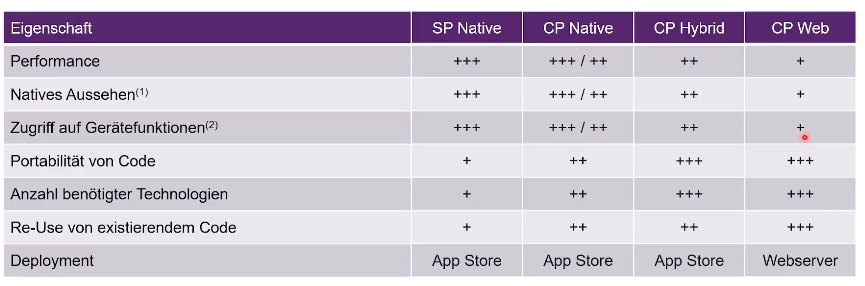
\includegraphics[width=.9\linewidth]{img/vor-nachteile-native-web-hybrid.png}
\end{center}

\textbf{AOSP}

Android is OpenSource and is called  \textbf{AOSP}.
Google and the other developers normally use the AOSP and add their own services on top of the System.
The problem is that if updates happen in the AOSP this often is not deployt to the end user.
This would be to much work for the big companies to update their system.
Often only big version changes / security patches are applied.
This is the reason for a big version fragmentation.

\textbf{Activity}

Activities are the basic building blocks for creating Android Apps.
One activity should only do one tasks.
The MainActicity is the first Activity started when the app is opened (similar to a main function in \href{../../../roam/20201116150053-java.org}{Java} / \href{../../../roam/20210921143046-kotlin.org}{Kotlin}).
The MainActivity is defined in the \href{../../../roam/20210921175054-androidmanifest.org}{AndroidManifest}.
An Activity consists of an XML-file (Layout) and a \href{../../../roam/20201116150053-java.org}{Java} / \href{../../../roam/20210921143046-kotlin.org}{Kotlin} file (logic). 

\textbf{Manifest}

The AndroidManifest.xml contains essential information over the app which are important for the operating system.
The most important parts of the file are:
\begin{itemize}
\item package: a unique ID for the app
\item versionName: human readable string. Mostly in the style of 1.0.0
\item versionCode: a positive Inter for internal usage. Higher number = new App. Can just be incremented
\item minSDKVersion: minimal required SDK Version the smartphone needs
\item maxSDKVersion: max required SDK (is ignored)
\item targetSDKVersion: on which SDK Version you tested your application
\end{itemize}

\textbf{Callbacks}

\begin{center}
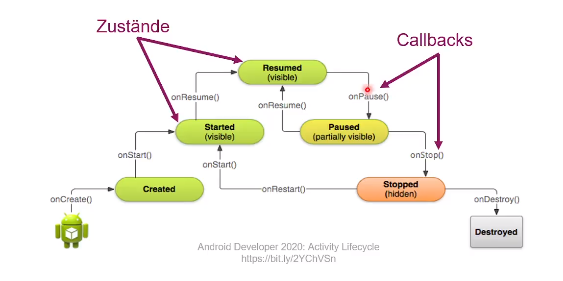
\includegraphics[width=.9\linewidth]{img/android_callbacks.png}
\end{center}


\textbf{Ressources}

Every Android App has some resources. It exist different kind of resources:
\begin{itemize}
\item colors which are used in the app (colors.xml)
\item strings which are used (strings.xml)
\item styles (styles.xml)
\item dimensions / sizes (dimens.xml)
\end{itemize}


To reference a value from one of the resource file the following syntax is used:
!!Source 1!!


\textbf{The R Class}

The \texttt{R} class in the \href{../../../roam/20210928175951-android_sdk.org}{Android SDK} is generated during the build.
With this class all the IDs of the \href{../../../roam/20210928180142-ressources_in_the_androids_sdk.org}{Ressources in the Androids SDK} can be access.
The ID is often used to get the Java / Kotlin element to interact with:
!!source 2!!

\textbf{Reach on Event}

To respond to a event \textbf{listeners} are used:
!!source 3!!

\textbf{Dimensions}

In the Android SDK exist six diffrent units for dimensions:
\begin{itemize}
\item dp: Density-indepentend pixels (das sollte man verwendend)
\item sp: scale-independend pixels (das verwenden, wenn man mit Schriftgrössen arbeitet)
\item px: Pixels
\item pt: Punkt
\item in: Inch
\item mm: millimeter
\end{itemize}


You should only use \texttt{dp} and \texttt{sp} because these two units are the only one which scale with the screen resolution.
\texttt{sp} should be used if it is used for text size because if the setting \texttt{big font size} is enabled on Android the font is scaled.
\texttt{dp} is not affected by \texttt{big font size} option.


\textbf{Intents}

Intents are used to call other components like an other Activity or an other App.
In the \href{../../../roam/20210928175951-android_sdk.org}{Android SDK} exists two diffrent kind of intents:
\begin{itemize}
\item \href{../../../roam/20211002180419-explicit_intents.org}{Explicit intents} (An explicit intent is mostly used to call an other component of the own app)
\item \href{../../../roam/20211002180703-implicit_intents.org}{Implicit intents} (An implicit intent is used mostly used call other apps)
\end{itemize}

An App can register itself for implicit intents inside the \href{../../../roam/20210921175054-androidmanifest.org}{AndroidManifest}.

To send data to the target component the following functions are used:
\begin{itemize}
\item \texttt{setData}
\item \texttt{putExtra() / putExtras()}
\end{itemize}


\textbf{Explicit Intent}

An explicit intent is mostly used to call an other component of the own app.
As an example to switch the activity:

!!source 4!!

\textbf{Implicit Intent}

An implicit intent is used mostly used call other apps.
For example when my app needs to take a picture it can ask the operating system to open an other app to take this photo.
Thanks to this concept not every app has to implement everything by itself.

It is important to check if a receiver is installed which can handle the intent.
If no receiver is installed and you send your intent, the app will crash with an exception.

!!source 5!!

\textbf{Gestartete Apps}
TODO


\textbf{AppComat / Compatibility}

AppCompat is a part of the Jetpack Library in the AndroidX namepace.
It is used to use new Features on old devices.
Where possible you should use the AppCompat class instead of the original \href{../../../roam/20210928175951-android_sdk.org}{Android SDK} version.


\textbf{Layouts}

The Simple Layouts are used when you know at compile time how many items should be rendered on the Screen.
In the \href{../../../roam/20210928175951-android_sdk.org}{Android SDK} exits multiple simple layouts. But today only the \href{../../../roam/20211017134616-jetpacks_constraintlayout.org}{Jetpacks ConstraintLayout} is used.
The most important attributes:
\begin{itemize}
\item \texttt{layout\_width}
\begin{itemize}
\item match\textsubscript{parent} (as big as possible)
\item match\textsubscript{content} (as small as possible)
\item dp (not recommended)
\end{itemize}
\item \texttt{layout\_height}
\begin{itemize}
\item match\textsubscript{parent} (as big as possible)
\item match\textsubscript{content} (as small as possible)
\item dp (not recommended)
\end{itemize}
\item \texttt{padding}
\item \texttt{layout\_margin}
\end{itemize}

The prefix \texttt{layout\_} indicates that the argument is just a wish to the parent view element.
The parent can ignore / adjust this option to optimize the screen.

\textbf{Linear Layout}

In the LinearLayout all children are arranged vertically or horizontally.


\begin{itemize}
\item \texttt{android:orientation=vertical}
\item \texttt{andoird:orientation=horizontal}
\item \texttt{android:layout\_weight=xx}
\begin{itemize}
\item the larger the number the wider the bar
\item use it only with \texttt{wrap\_content}
\end{itemize}
\end{itemize}

\begin{center}

\includegraphics[width=.9\linewidth]{img/linearlayout.png}
\end{center}

\textbf{FrameLayout}

In the FrameLayout the children are stacked on each other.
As an example a photo app, in the background the live image and on top the control widgets. 


Adjustment in the height:
\begin{itemize}
\item the later in the XML the higher the control
\item set the height manually with \texttt{android:translationZ}
\end{itemize}


\begin{center}
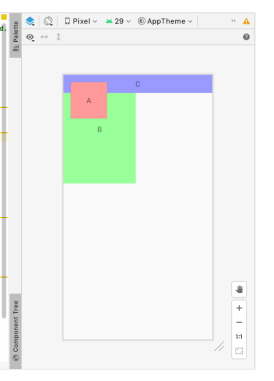
\includegraphics[width=.9\linewidth]{img/framelayout.png}
\end{center}

\textbf{RelativeLayout}

In the RelativeLayout the elements are arranged relatively to each other.
This is often used for a efficient alternative for nested Layouts (\href{../../../roam/20211017141728-nested_layouts_in_android.org}{Nested Layouts in Android}).

\textbf{Jetpacks ConstraintLayout}

Today the ConstraintLayout should be used for \href{../../../roam/20211017133750-the_simple_layouts_in_android.org}{The Simple Layouts in Android}.
The ConstraintLayout is similar to the RelativeLayout (\href{../../../roam/20211017135008-the_relativelayout_in_android.org}{The RelativeLayout in Android}).
The whole Screen is designed using constraints.

Android Studio generated good code (XML) for the ConstraintLayout.
The size \texttt{0dp} means that the size should be calculated from the constraints.

The ConstraintLayout is \textbf{not} in the \texttt{android:} namespace.
It is in the XML namespace \texttt{app:}. 


\textbf{Adapter Layout}
The AdapterLayout can render a potential infinite set of information.
It is not known how many items are available during compile time.
For this the \href{../../../roam/20211017144845-jetpacks_recyclerview.org}{Jetpacks RecyclerView} is used.

The RecyclerView is an element from the Jetpack Library (\href{../../../roam/20211112094119-android_jetpack.org}{Android Jetpack}).
As the name says it recycles views (\href{../../../roam/20211017133835-the_adapter_layouts_in_android.org}{The Adapter Layouts in Android}).

You have to implement a ViewHolder and an Adapter
The ViewHolder inherits from \texttt{RecyclerView.ViewHolder} and stores the reference to the view elements.
The Adapter inherits from \texttt{RecyclerView.Adapter<T>} is used to build from the data an appropriate view.
The Adapter must override the following functions:
\begin{itemize}
\item \texttt{onCreateViewHolder()}: creates a new ViewHolder with references
\item \texttt{onBindViewHolder()}: attach new content to the ViewHolder
\item \texttt{getItemCount()}: the size of the underlying collection
\end{itemize}


\begin{center}
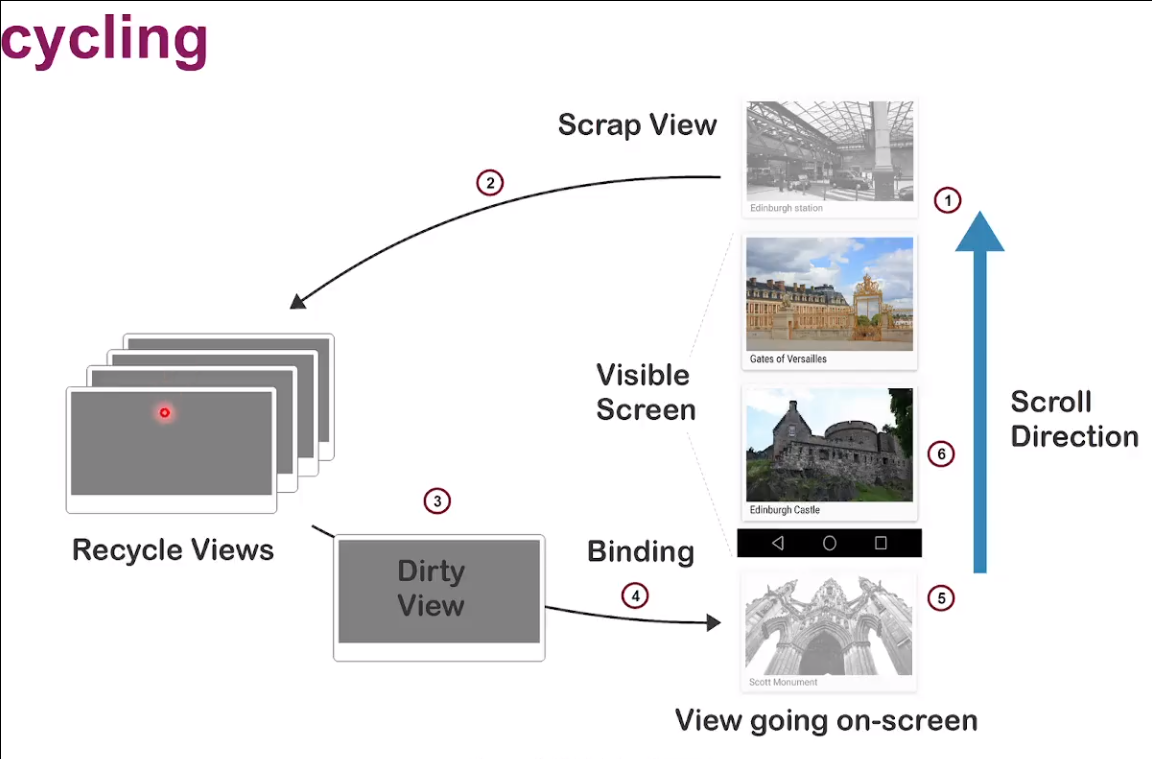
\includegraphics[width=.9\linewidth]{img/view_recycling.png}
\end{center}

\textbf{Nested Layout}
But this should be avoided if possible because this has massive negative impacts on the performance.
\emph{Wide and flat hierarchy}.

\textbf{Widgets}

All Widgets in the \href{../../../roam/20210928175951-android_sdk.org}{Android SDK} are in the Namespace \texttt{android.widget} and inherit from \texttt{View}.

\begin{itemize}
\item TextView
\item Imageview
\item Button
\item ImageButton
\item EditText
\item Checkboxes
\item Picker (for Example Date picker)
\item Floating Action Button (often place at the bottom)
\item Radio Buttons
\item Seek  Bar (slider bar)
\item Switches
\item Rating Bar
\item Spinne (Combobox / Dropdown)
\end{itemize}


There exits also UI-Widget with out XML. These widgets are generated from the OS over an API.
\begin{itemize}
\item Toasts
\item Snackbars
\item Dialoge
\item Notifications
\end{itemize}

\textbf{Fragments}

Sometimes you want to use the same screen in multiple activities.
For example a list of items which is faded in.
This list of item can not be implemented as a \href{../../../roam/20210921174424-android_sdk_activity.org}{Android SDK Activity}.
But with a \textbf{Fragment} it is possible.
A fragment consists of a XML and Java file.

Use only the \texttt{androidx.fragment.app*} classes.


\begin{center}
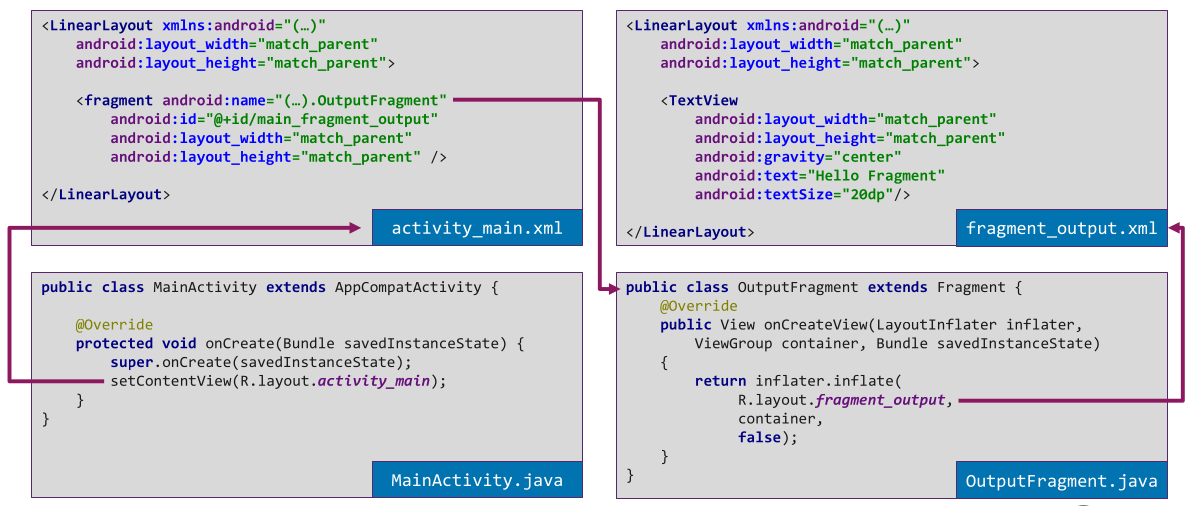
\includegraphics[width=.9\linewidth]{img/fragment_static_include.png}
\end{center}

\begin{center}
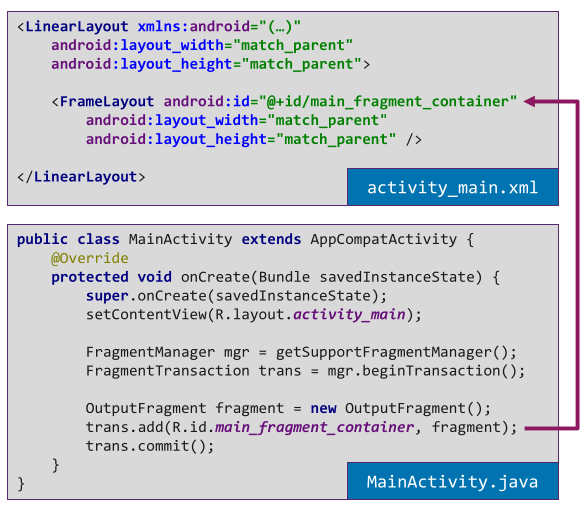
\includegraphics[width=.9\linewidth]{img/fragment_dynamic_include.png}
\end{center}

\begin{center}
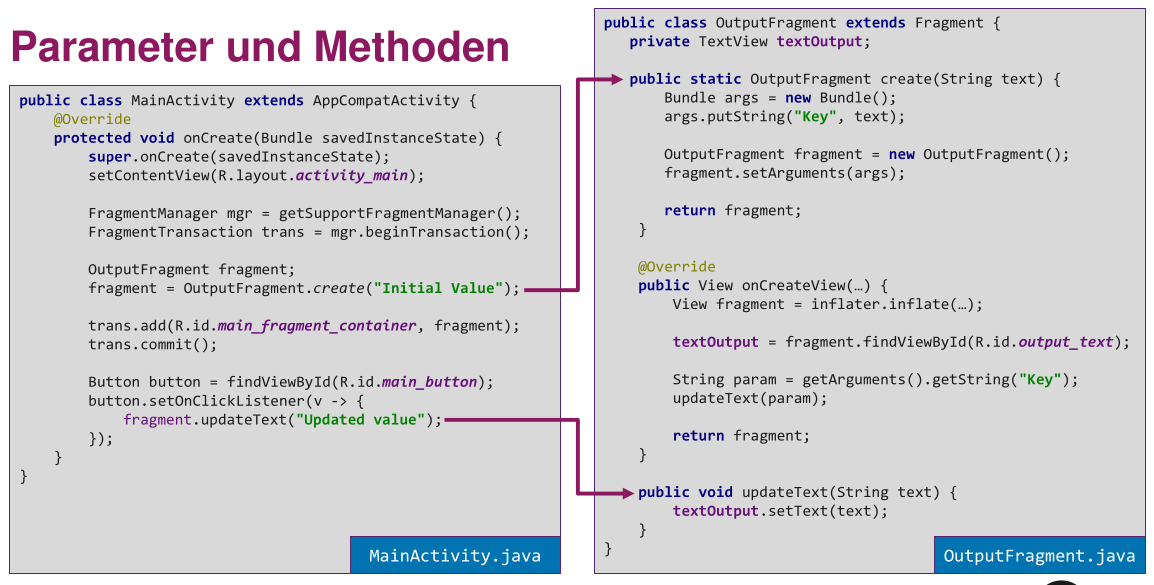
\includegraphics[width=.9\linewidth]{img/fragment_parameter_method.png}
\end{center}


\textbf{How to hand over parameters to a fragment}

Use always \texttt{Bundle} to set parameters for the Fragment (\href{../../../roam/20211023174645-what_are_fragments_in_the_android_sdk.org}{What are Fragments in the Android SDK})
Otherwise, the values getting lost when the fragment is updated.
It is recommended to create a Factory Function to create the fragment.
!!source 6!!


\textbf{Styles in Android}

\begin{center}
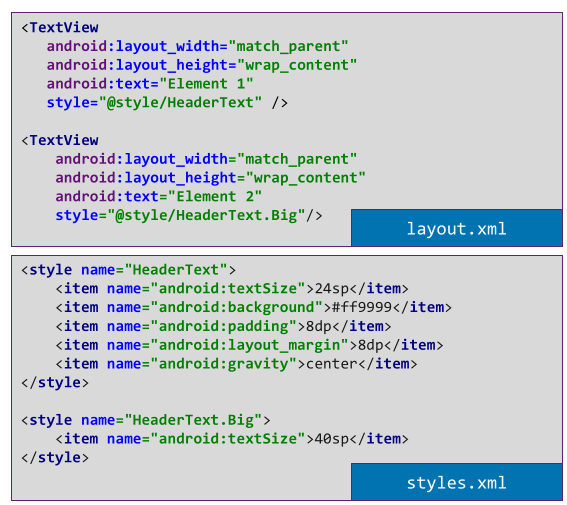
\includegraphics[width=.9\linewidth]{img/styling_in_the_android_sdk.png}
\end{center}

\begin{center}
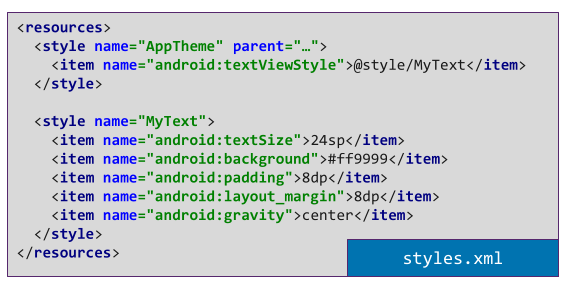
\includegraphics[width=.9\linewidth]{img/theme_definition.png}
\end{center}

\begin{center}
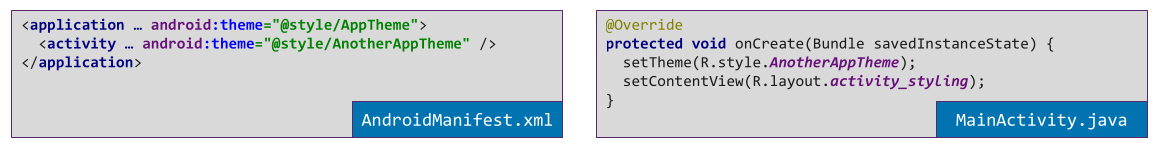
\includegraphics[width=.9\linewidth]{img/use_themes_in_android.png}
\end{center}


\textbf{Material Design}

Material is the metaphor:
\begin{itemize}
\item inspired by the pysical world
\item surface should be like paper and ink
\end{itemize}

Bold, graphic, intentional:
\begin{itemize}
\item based on prinicples of print medias
\item hierarchy, grid, fonts, colors
\end{itemize}

Motion provides meaning:
\begin{itemize}
\item motion means action
\item sestrained, subtle use
\end{itemize}


\textbf{Permissions}

In Android exists two kinds of permission:
\begin{itemize}
\item normal, requested by the system
\item dangerous, requested by the user
\end{itemize}

Permissions can be revoked by the user at \textbf{any} time.
Since API 30 it is possible that the system revokes the permission automatically.
\textbf{Important}: Check always access on proceeded APIs.
If not a \texttt{SecurityException} could be thrown.


\textbf{Persistence}

In Android exits 5 APIs to store something on the storage:

\begin{itemize}
\item App-sepcific files
\begin{itemize}
\item anything
\item internal / external
\item File API
\end{itemize}
\item Preferences
\begin{itemize}
\item Key-Value, simple value
\item internal
\item SharedPreferences
\end{itemize}
\item Database
\begin{itemize}
\item often domainobjects
\item internal
\item SQLite / Room
\end{itemize}
\item Medien
\begin{itemize}
\item Images, Videos, Music
\item external
\item MediaStore
\end{itemize}
\item Dokumente
\begin{itemize}
\item Documents (PDF, ZIP)
\item external
\item Storage Access Framework
\end{itemize}
\end{itemize}


\textbf{Sensor Framework}

For accessing the sensors in a Android based smartphone you use the Sensor Framework.
All sensors use the same API:
\begin{itemize}
\item \texttt{SensorManager}, entry point
\item \texttt{Sensor}, represent the real sensor
\item \texttt{SensorEvent}, contains the values
\item \texttt{SensorEventListener}, used for callbacks
\end{itemize}


\textbf{Layer Architecture}

\begin{center}
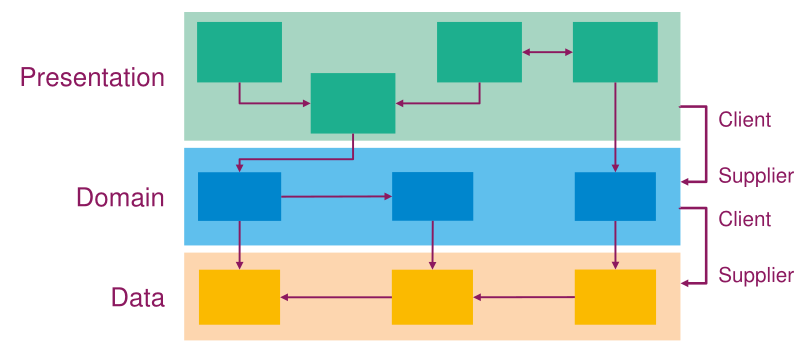
\includegraphics[width=.9\linewidth]{img/layer_architecture.png}
\end{center}


\textbf{Obeserver Pattern}

The goal of the Observer Pattern is to resolve a cyclic dependency.
The Pattern consists of two objects:

\begin{itemize}
\item \emph{Subject}: is monitored (e.g. a model)
\item \emph{Observer}: monitors the subject (e.g. a view)
\end{itemize}


The observer register it self on the subject.
The only requirement is that the subject implements a specific interface (\href{../../../roam/20201116150053-java.org}{Java}, \href{../../../roam/20211003114158-c.org}{C\#}).
Using this approach the domain does not have to need anything from the view (excepted the interface).

\textbf{MVC}

The MVC consist of three parts:
\begin{itemize}
\item \emph{Model}: contains the data
\item \emph{View}: reads data from the model and render it
\item \emph{Controller}: coordination between View and Model
\end{itemize}


\begin{center}
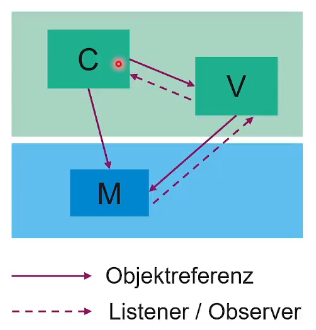
\includegraphics[width=.9\linewidth]{img/mvc.png}
\end{center}


\textbf{Application class}

Every Android App has a \texttt{application} node in the \href{../../../roam/20210921175054-androidmanifest.org}{AndroidManifest} file.
During the start of the app a instance of the class is created.
It is possible to inherit from this class.

!!source 7!!

Using a custom application class you can:
\begin{itemize}
\item create object which should be initialized only once
\item creating Singleton objects
\item access to global objects
\item monitor life cycle of all activities
\begin{itemize}
\item implemented interface
\end{itemize}
\end{itemize}

\textbf{Application Lifce Cycle}

\href{../../../roam/20211103155952-the_application_class_in_the_android_sdk.org}{The Application class in the Android SDK} has several life cycle methods:

\begin{itemize}
\item onCreate
\item onTerminate
\begin{itemize}
\item on real devices never called
\end{itemize}
\item onConfigurationChanged
\begin{itemize}
\item on system configuration changes
\end{itemize}
\item onLowMemory
\begin{itemize}
\item hint for a possible termination of the app
\end{itemize}
\item onTrimMemory
\begin{itemize}
\item on moments where it is possible to clean up
\item e.g. app is in background
\end{itemize}
\end{itemize}


\textbf{Context}

With a \texttt{Context} object it is possible to get access to various services and resources of an app.
Every \texttt{Context} object has a limited life time.
After the life time is over all resources requested by the context are freed. 


\emph{Attention}: The Application context has only restricted possibilities for UI interactions 
\begin{center}
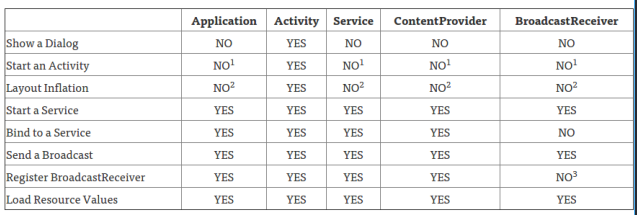
\includegraphics[width=.9\linewidth]{img/context_and_their_possibilities.png}
\end{center}


\textbf{Broadcasts}

Broadcasts are normal intents (\href{../../../roam/20211002175222-what_is_an_intent_and_for_what_it_is_used_in_the_android_sdk.org}{What is an Intent and for what it is used in the Android SDK?}) and are used to exchange message between apps.
There are two kinds of Broadcasts:
\begin{itemize}
\item lokal broadcasts: exchange inside the app
\item global broadcasts: \href{../../../roam/20211103165118-global_broadcasts_in_android.org}{Global Broadcasts in Android}
\end{itemize}

You can register your self for a broadcast (\href{../../../roam/20211029100710-what_are_broadcasts_in_android.org}{What are Broadcasts in Android?}) in two ways:
\begin{itemize}
\item statically in the \href{../../../roam/20210921175054-androidmanifest.org}{AndroidManifest} (not recommended / deprecated)
\item dynamically in the code (\href{../../../roam/20211103170117-dynamic_registration_for_broadcasts_in_android.org}{Dynamic registration for Broadcasts in Android})
\end{itemize}

\textbf{Global Broadcast}

Global broadcasts are used to exchange messages inside the whole system.
Android it self sends global broadcasts. For example when:
\begin{itemize}
\item the system is booted
\item network connection is lost
\item a SMS is received
\end{itemize}


\textbf{Services}

In Android (\href{../../../roam/20210921143632-aosp.org}{Android Open Source Project}) Services are used to start Tasks in the background.
For example:
\begin{itemize}
\item download data from a web page
\item play music
\end{itemize}


The Services is executed by the \textbf{Main-Thread}.
\emph{Important}: The lifecycle of a service is independent of the App and has no UI (some times a Notification).

\textbf{Started Service}

Started Services is one type of Services (\href{../../../roam/20211109103648-for_what_are_services_used_in_android.org}{For what are Services used in Android?}) in Android (\href{../../../roam/20210921143632-aosp.org}{Android Open Source Project}).
This kind of service is used for unique actions for example for a download of files from a webpage.

\emph{Attention}: This service runs potential for ever.

To stop the service:
\begin{itemize}
\item stopped by service itself: \texttt{stopSelf()}
\item stopped by application: \texttt{stopService()}
\item stopped by Android
\end{itemize}

\textbf{Bound Service}

Bound Services is one kind of services (\href{../../../roam/20211109103648-for_what_are_services_used_in_android.org}{For what are Services used in Android?}) in Android (\href{../../../roam/20210921143632-aosp.org}{Android Open Source Project}).
It is used for task which are long lasting.
For example a music player.

The communication between the app and the service is similar to a client/server communication.
The service can have multiple clients.
If the last client disconnects from the service it is stopped. 

\textbf{APK Files}

In Android (\href{../../../roam/20210921143632-aosp.org}{Android Open Source Project}) Apps are installed from a so called APK file (Android Package).
This APK files are just a normal zip file.

\textbf{APK Splitting}

In the Google Play Store the size of the APK file (\href{../../../roam/20211109113541-what_is_a_apk_file.org}{What is a APK file?}) is limited to 100 MB.
To overcome this limitation you can split your APK file in multiple smaller APKs

\textbf{APK Expansion Files}

In the Google Play Store the size of the APK file (\href{../../../roam/20211109113541-what_is_a_apk_file.org}{What is a APK file?}) is limited to 100 MB.
To overcome this limitation you can move your resources (e.g. videos) in a Exapnsion File (.OBB).
Play Store allows 2x2GB.

\textbf{What is the ABB?}

The Android App Bundle (AAB) is the successor of the APK (\href{../../../roam/20211109113541-what_is_a_apk_file.org}{What is a APK file?}).
AAB is a container for all the content from your app. You upload the the Container and \href{../../../roam/20211111145536-google.org}{Google} builds the APK dynamically. 

\begin{center}
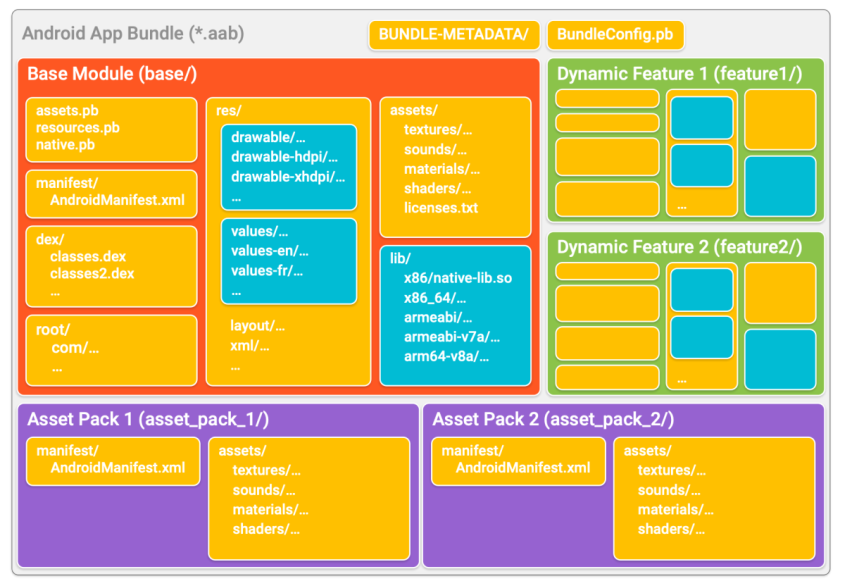
\includegraphics[width=.9\linewidth]{img/android_app_bundle.png}
\end{center}

\textbf{Android Build Process}

First all files from the project must be compiled to a APK file (\ref{org9e067aa}).
The resulting APK file (\href{../../../roam/20211109113541-what_is_a_apk_file.org}{What is a APK file?}) is uploaded to the Google Play Store.
The Installed App is executed.
If the code is already translated to Machine Code it is executed straight away.
Else you compile it to and upload the compiled part to the Play Store.
Next time a user needs this part of code is does not need to compile it by itself (\ref{org8248bda}). 

\begin{center}
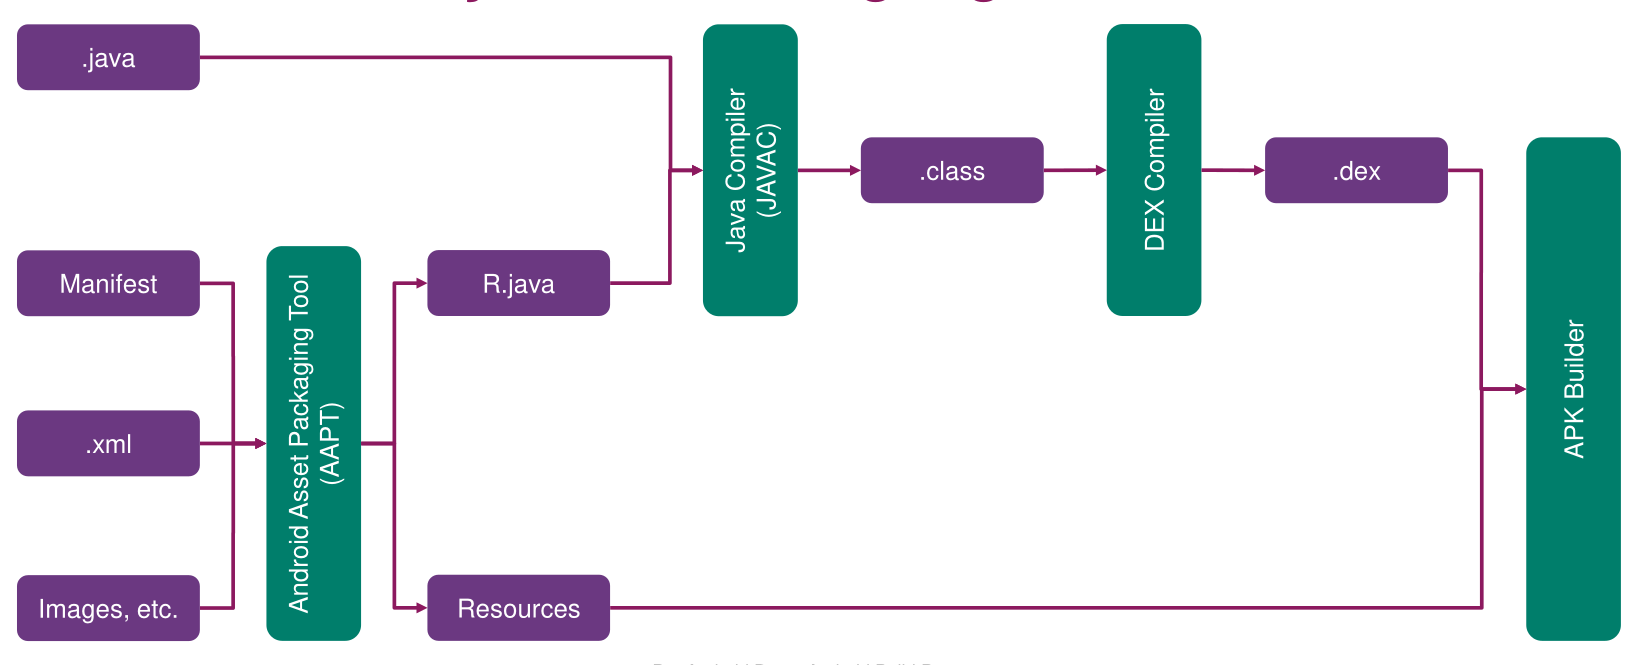
\includegraphics[width=.9\linewidth]{img/android_build_system_create_apk.png}
\label{org9e067aa}
\end{center}


\begin{center}
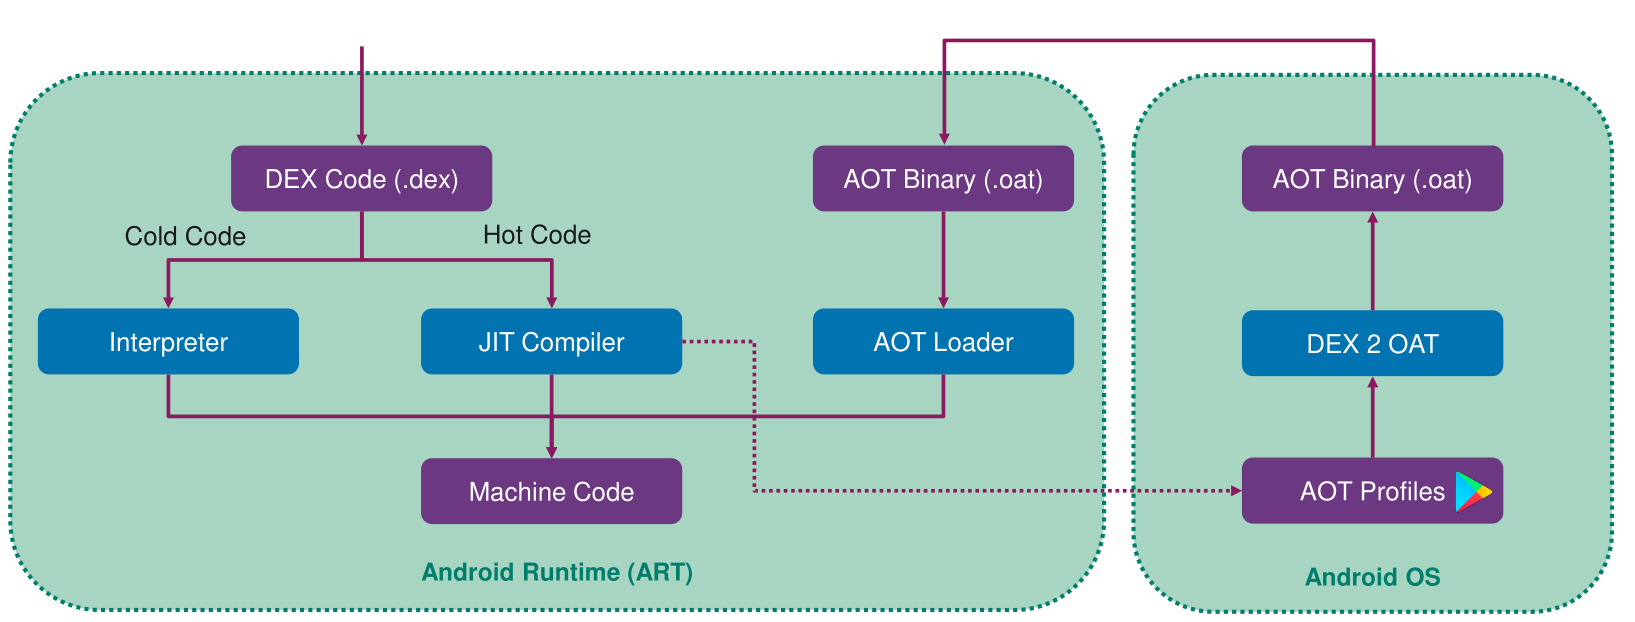
\includegraphics[width=.9\linewidth]{img/android_build_system_art_2_0.png}
\label{org8248bda}
\end{center}

\textbf{View Binding}

View Binding is way to access the View Elements. It's benefit over the traditional way are:
\begin{itemize}
\item type safety
\item null safety
\item no \texttt{findViewById()} calls
\end{itemize}


View Binding (\href{../../../roam/20211112094953-what_is_view_binding_in_an_android_application.org}{What is View Binding in an Android Application?}) needs to be enabled in \href{../../../roam/20211112095502-gradle.org}{Gradle}.
The Binding class is generated during the build.
The name of the Binding class is build from the Layout name in Camel Case with \texttt{Binding} as suffix:
\begin{itemize}
\item \texttt{activity\_main.xml} \(\rightarrow\) \texttt{ActivityMainBinding}
\end{itemize}

\textbf{Data Binding}

With Data Binding you can access data from inside the \href{../../../roam/20211112100344-xml.org}{XML}.
This is achieved with the \href{../../../roam/20211103140808-observer_pattern.org}{Observer Pattern}.
The Layout is the Observer of the Data.

Data Binding (\href{../../../roam/20211112100504-what_is_data_binding_in_an_android_application.org}{What is Data Binding in an Android Application?}) has to be enabled in the \href{../../../roam/20211112095502-gradle.org}{Gradle} settings.
If you want to observe your class see \href{../../../roam/20211112103257-how_to_make_your_class_observable_for_data_binding.org}{How to make your Class observable for Data Binding?}. 

\textbf{How to make Class Observable}

\emph{Attention}: A object witch is used with Data Binding (\href{../../../roam/20211112100504-what_is_data_binding_in_an_android_application.org}{What is Data Binding in an Android Application?}) is \emph{not} automatically observable.
You have to change the data source in the following way:
\begin{itemize}
\item \emph{observable fields}:  this should be used for a few values only
\item \emph{observable objects}: this should be used if the whole class should be observed
\begin{itemize}
\item you have to mark with the Annotation \texttt{@Bindable} the getters.
\end{itemize}
\end{itemize}


\textbf{How to bind an Event}

First you have to enable Data Binding (\href{../../../roam/20211112101553-how_to_use_data_binding_in_your_android_application.org}{How to use Data Binding in your Android Application?}).
Then you have two options:
\begin{itemize}
\item \emph{method references}: references directly to the function with a fitting signature
\item \emph{listener bindings}: allows the usage of expressions before making a call
\end{itemize}


\textbf{One-way vs. two-way}

A One-Way binding is Data Binding (\href{../../../roam/20211112100504-what_is_data_binding_in_an_android_application.org}{What is Data Binding in an Android Application?}) or View Binding (\href{../../../roam/20211112094953-what_is_view_binding_in_an_android_application.org}{What is View Binding in an Android Application?}) exclusive.
You only use one of them.
But often you want a Two-Way Binding.
If the data changes the view changes, and if the user changes the UI the data are changed.

\textbf{Risk of Data Binding}

Common risks with Data Binding (\href{../../../roam/20211112100504-what_is_data_binding_in_an_android_application.org}{What is Data Binding in an Android Application?}):
\begin{itemize}
\item Pollute the the Model with \href{../../../roam/20210928175951-android_sdk.org}{Android SDK} Details
\item to much logic in the layout
\item difficult to debug
\item takes longer for the compilation (I think that is not that bad)
\item possible occurrence of invisible observers (\href{../../../roam/20211112110032-what_is_a_invisible_observer.org}{What is a Invisible Observer?})
\end{itemize}


\textbf{MVVM}

The MVVM Pattern consists of three parts:
\begin{itemize}
\item \emph{Model}: contains the Domain / business logic
\item \emph{View}: contains the graphical UI and user input
\item \emph{View Model}: contains the logic form the UI and ensures the communication between Model and View
\begin{itemize}
\item This is often achived over Data Binding
\item \href{../../../roam/20211112100504-what_is_data_binding_in_an_android_application.org}{What is Data Binding in an Android Application?}
\item \href{../../../roam/20211207163530-data_binding_in_wpf.org}{Data Binding in WPF}
\end{itemize}
\end{itemize}


The benefits of the MVVM pattern are:
\begin{itemize}
\item View Model is easy to test because it does not contain any UI classes
\item the View has only visual tasks
\item Changes in the Model do not directly affect the View
\end{itemize}

\begin{center}
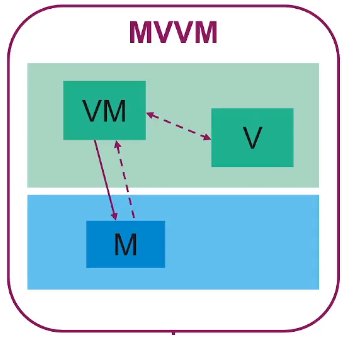
\includegraphics[width=.9\linewidth]{img/mvvm.png}
\end{center}


\textbf{Lifecycle Aware Component}

A Lifecycle Aware Component reacts on state changes of \textbf{a other component}.
Using this approach the state logic moves from the owner to the observer.

To implement a Lifecylce Aware Component you need two concepts:
\begin{itemize}
\item \emph{LifecylceOwner}: manage the state in a \texttt{Lifecylce} object
\item \emph{LifecylceObserver}: observes the Lifecycle object (and with this the LifecylceOwner)
\end{itemize}


\textbf{LiveData Class}
LiveData is a lifecycle-aware observable (\href{../../../roam/20211112114814-what_is_a_lifecycle_aware_component.org}{What is a Lifecycle Aware Component?}, \href{../../../roam/20211103140808-observer_pattern.org}{Observer Pattern}) from the \href{../../../roam/20210928175951-android_sdk.org}{Android SDK}.
The benefit that is also solves the Invisible Observer Problem (\href{../../../roam/20211112110032-what_is_a_invisible_observer.org}{What is a Invisible Observer?}).

It's an alternative to Observable Fields / Observable Objects (\href{../../../roam/20211112103257-how_to_make_your_class_observable_for_data_binding.org}{How to make your Class observable for Data Binding?}) and is possible to use it as a source for Data Binding (\href{../../../roam/20211112100504-what_is_data_binding_in_an_android_application.org}{What is Data Binding in an Android Application?})
The Observer is notified if enabled and are removed if it is stopped (\href{../../../roam/20211112110032-what_is_a_invisible_observer.org}{What is a Invisible Observer?})
\end{multicols}

\section{Code}
\label{sec:orgab9ac94}
\textbf{Source 1 - Access Value from Resource}

\lstset{language=XML,label= ,caption= ,captionpos=b,numbers=none}
\begin{lstlisting}
<Button
    android:id="@+id/buttonNavigate" <!-- creates new ID on place -->
    android:text="@string/open_2nd_activity" <!-- references open_2nd_activity in strings.xml --> />
\end{lstlisting}

\textbf{Source 2 - R Class example}

\lstset{language=java,label= ,caption= ,captionpos=b,numbers=none}
\begin{lstlisting}
var button = (Button)this.findViewById(R.id.btnLogIn);
\end{lstlisting}

\textbf{Source 3 - Reach on an Event using listeners}

\lstset{language=java,label= ,caption= ,captionpos=b,numbers=none}
\begin{lstlisting}
final TextView textView = this.findViewById(R.id.text_example);
Button button = this.findViewById(R.id.button_example);

button.setOnClickListener(new View.OnClickListener() {
	@Override
	public void onClick(View view) {
	    textView.setText("Button pressed");
	}
    }
 );

// Java 8 (Lambda)
button.setOnClickListener(v -> { /**/ });
\end{lstlisting}

\textbf{Source 4 - Explicit Intent}

\lstset{language=kotlin,label= ,caption= ,captionpos=b,numbers=none}
\begin{lstlisting}
// SecondActivity.kt
class SecondActivity : AppCompatActivity() {
    companion object {
	private const val MESSAGE_KEY = "MESSAGE";
	fun createIntent(context: Context, message: String): Intent {
	    val intent = Intent(context, SecondActivity::class.java)
	    intent.putExtra(MESSAGE_KEY, message)
	    return intent
	}
    }

    override fun onCreate(savedInstanceState: Bundle?) {
	super.onCreate(savedInstanceState)
	setContentView(R.layout.activity_second)

	val textBox = findViewById<TextView>(R.id.textOutput)
	val message = intent.extras?.getString(MESSAGE_KEY)
	textBox.text = message
    }
}

// Some other activity
startActivity(SecondActivity.createIntent(this, "Hallo Welt"))
\end{lstlisting}

\textbf{Source 5 - Implicit Intent}

\lstset{language=java,label= ,caption= ,captionpos=b,numbers=none}
\begin{lstlisting}
val intent = Intent(Intent.ACTION_VIEW, Uri.parse("https://www.ost.ch"))
val hasReceiver = intent.resolveActivity(getPackageManager()) != null;
\end{lstlisting}

\lstset{language=XML,label= ,caption= ,captionpos=b,numbers=none}
\begin{lstlisting}
<uses-permission android:name="android.permission.QUERY_ALL_PACKAGES" />
\end{lstlisting}

\textbf{Source 6 - Fragment with parameters}

\lstset{language=java,label= ,caption= ,captionpos=b,numbers=none}
\begin{lstlisting}
public class OutputFragment extends Fragment {
    private TextView textOutput;
    public static OutputFragment create(String text) {
	Bundle args = new Bundle();
	args.putString("Key", text);
	OutputFragment fragment = new OutputFragment();
	fragment.setArguments(args);
	return fragment;
    }
}
\end{lstlisting}

\textbf{Source 7 - The application class}

\lstset{language=XML,label= ,caption= ,captionpos=b,numbers=none}
\begin{lstlisting}
<application android:name=".MyApplication">
  <!-- Ower Components -->
</application>
\end{lstlisting}

\lstset{language=java,label= ,caption= ,captionpos=b,numbers=none}
\begin{lstlisting}
public class MyApplication extends Application {
    @Override
    public void onCreate() {
	super.onCreate();
    }

    // .. more callbacks
}
\end{lstlisting}
\end{document}